\documentclass[11pt]{article}

\usepackage{amsfonts}
\usepackage{graphicx}
\usepackage{amssymb}
\usepackage{tikz}
\usepackage{amsmath}
\usetikzlibrary{arrows}
\usepackage{pgfplots}
\pgfplotsset{compat=1.7}

\begin{document}
	\noindent \begin{huge}Kirill Beskorovainyi. Hausaufgabe 2:\end{huge}\\\vspace{0.05in}

		\noindent \begin{Large}Aufgabe 1:\end{Large}\\[2pt]
			\indent a)\\
				Induktionsanfang: Für $n=1$
					$$\sum\limits_{k=1}^1 (2k-1)=2 \times 1 - 1 = 1$$
					$$1^2=1$$
					$$1 = 1$$
				Induktionsvoraussetzung:\\
				Für ein belibiges, aber festes $n \in \mathbb{N}$, $n \geq 1$ gelte:
					$$\sum\limits_{k=1}^n(2k-1)=n^2$$
				Induktionsbehauptung:\\
				Dann gilt auch:
				$$\sum \limits_{k=1}^{n+1}(2k-1)=(n+1)^2$$
				\underline{(IV:)} \\
					$$\sum\limits_{k=1}^{n+1}(2k-1)=\sum\limits_{k+1}^{n}(2k-1)+2(n+1)-1=$$
					$$=(n^2)+2n+1 = (n+1)^2$$

			\indent b)\\
				Induktionsanfang: Für $n=2$
					$$\prod\limits_{k=2}^2(1-\frac{1}{2^2})=\frac{3}{4}$$
					$$\frac{2+1}{2\times2}=\frac{3}{4}$$
					$$\frac{3}{4}=\frac{3}{4}$$
				Induktionsvoraussetzung:\\
				Für ein belibiges, aber festes $n \in \mathbb{N}$, $n \geq 2$ gelte:
					$$\prod\limits_{k=2}^n(1-\frac{1}{k^2})=\frac{n+1}{2n}$$
				Induktionsbehauptung:\\
				Dann gilt auch:
					$$\prod\limits_{k=2}^{n+1}(1-\frac{1}{k^2})=\frac{n+2}{2(n+1)}$$
				\underline{(IV:)} \\
					$$\prod\limits_{k=2}^{n+1}(1-\frac{1}{k^2})=\prod\limits_{k=2}^n(1-\frac{1}{k^2})\times(1-\frac{1}{(n+1)^2})=\left(\frac{n+1}{2n}\right)\times\left(1-\frac{1}{(n+1)^2}\right)=$$
					$$=\frac{n+1}{2n}-\frac{n+1}{2n(n+1)^2}=\frac{(n+1)^2-1}{2n(n+1)}=$$
					$$=\frac{n^2+2n}{2n(n+1)}=\frac{n+2}{2(n+1)}$$
			\indent c)\\
				Induktionsanfang: Für $n=4$
					$$2^4 = 16$$
					$$4^2 = 16$$
				Induktionsvoraussetzung:\\
				Für ein belibiges, aber festes $n \in \mathbb{N}$, $n \geq 4$ gelte:
					$$2^n \geq n^2$$
				Induktionsbehauptung:\\
				Dann gilt auch:
					$$2^{n+1}\geq (n+1)^2$$
				\underline{(IV:)} \\
					$$2^{n+1}=2^1 \times 2^n=2^n+2^n$$
					Aus Induktionsvoraussetzung: $2^n \geq 2^n$, also $2 \times 2^n \geq 2 \times 2^n$
					$$2^n+2^n \geq n^2+n^2 \geq n^2+n \times n$$
					
					$$n\geq4 => 2^{n+1} \geq n^2+4n$$
					$$\geq n^2 + 2n + 2n$$
					$$\geq n^2 + 2n + 2(4)$$
					$$\geq n^2 + 2n + 1 \geq (n+1)^2$$\\
				Teil 2:\\
				Für $n=0,1,2,3$	\\
				\begin{tikzpicture}
				\begin{axis}[
				    axis lines = middle,
				    xmin=-2,xmax=6,ymin=0,ymax=20,
				    xlabel = $n$,
   					ylabel = {$f(n)$},
]
%Below the red parabola is defined
				\addplot [
				    domain=-2:6, 
				    samples=100, 
				    color=red,
]
				{x^2};
				\addlegendentry{$n^2$}
				\addplot [
				    domain=-2:6, 
				    samples=100, 
				    color=blue,
]
				{2^x)};
				\addlegendentry{$2^n$}
			\end{axis}
			\end{tikzpicture}\\
			Für $[0,2]$ ist $2^n \geq n^2$, aber für $[2,4]$ ist $2^n \leq n^2$\\
			Also die Aussage gilt für $n=0,1,2$, aber nicht für $n=3$\\
		\noindent \begin{Large}Aufgabe 2:\end{Large}\\[2pt]
			\indent a) $f: \mathbb{R} \rightarrow \mathbb{R}$, $x \mapsto 2e^x$\\
			\begin{tikzpicture}
				\begin{axis}[
				    axis lines = middle,
				    xmin=-2,xmax=2,ymin=-0.5,ymax=5,
				    xlabel = $x$,
   					ylabel = {$f(x)$},
]
%Below the red parabola is defined
				\addplot [
				    domain=-2:2, 
				    samples=100, 
				    color=red,
]
				{2*(pow(2.71828,x)};
				\addlegendentry{$2e^x$}
			\end{axis}
		\end{tikzpicture}\\
			Seien $x_1, x_2 \in \mathbb{R}$ mit:
				$$f(x_1)=f(x_2)$$
				$$2e^{x_1}=2e^{x_2}$$
				$$e^{x_1}=e^{x_2}$$
				$$x_1=x_2$$
				$$\mbox{Damit }f \mbox{ ist \underline{injektiv}.}$$
				Angenommen, es existiert ein $x \in D_f$, sodass $f(x)=-1$. Dann wäre aber $-1=f(x)=2e^x>0$, was einen Wiederspruch darstellt. Daher ist $-1$ nicht im Bild von $f$ und $f$ ist \underline{nicht surjektiv}.\\
				Da $f$ injektiv, aber nicht surjektiv ist, kann sie \underline{nicht bijektiv} sein.\\
			\indent b) $g: \mathbb{R} \rightarrow \mathbb{R}$, $x \mapsto \mid x \mid ^3$\\
				\begin{tikzpicture}
					\begin{axis}[
					    axis lines = middle,
					    xlabel = $x$,
	   					ylabel = {$f(x)$},
]
%Below the positive parabola is defined
					\addplot [
					    domain=-2:0, 
					    samples=100, 
					    color=red,
]
					{-x^3};
%Below the negative parabola is defined
					\addplot [
					    domain=0:2, 
					    samples=100, 
					    color=red,
]	
					{x^3};
					\addlegendentry{$\mid x \mid ^3$}
				\end{axis}
			\end{tikzpicture}\\
				Die Fuktion ist \underline{nicht injektiv}, da $g(-1)=1=g(1)$, aber $1 \neq -1$.\\
				Angenomen, es existiert ein $x \in D_f$, sodass $f(x)=-2$. Dann wäre aber $-2=f(x)= \mid x \mid ^3 \geq 0$, was einen Wiederspruch darstellt. Daher ist $-2$ nicht im Bild von $g$ und $g$ ist \underline{nicht surjektiv}.\\
				Da $g$ weder injektiv noch surjektiv ist, ist sie \underline{nicht bijektiv}.\\
		\noindent \begin{Large}Aufgabe 3:\end{Large}\\[2pt]
			\indent a) 
				$f_1(x)=x^2-4$ ist ein Polynom 2. Grades und im ganzen $\mathbb{R}$ definiert.\\ Also:
				$$D_{f_1} = \mathbb{R}$$
				$f_2(x)=\frac{1}{x^3}$ ist nur dann definiert, wenn $x^3 \neq 0$, also $x \neq 0$:\\Daher ist:
				$$D_{f_2} = \mathbb{R}^{\neq 0}$$
				$f_3(x) = \frac{sin(x)}{cos(x)} = tan(x)$ ist $\pi$-periodisch, d.h. $tan(\phi + k\pi)=tan(\phi)$ für alle $\phi \in \mathbb{R} \setminus \{\frac{\pi}{2}+k\pi \mid k \in \mathbb{Z}\}$\\
				Somit ist:
				$$D_{f_3} = \{x \in \mathbb{R} \mid x \neq \frac{\pi}{2}+k \pi \mbox{, } k \in \mathbb{Z}\}$$
				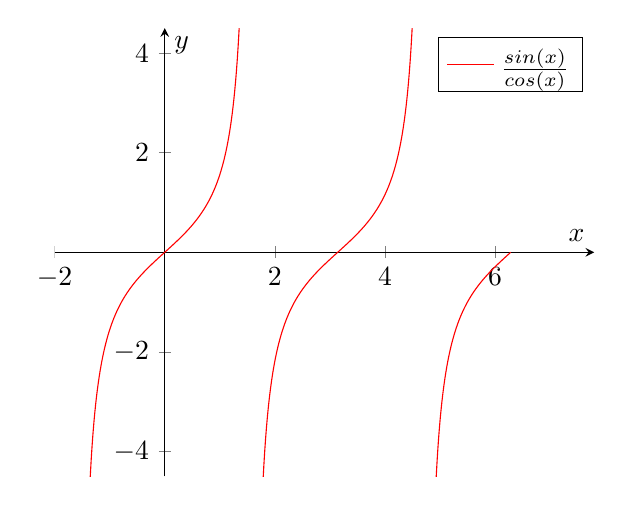
\begin{tikzpicture}
					\begin{axis}[
					    axis lines=middle,
   						xmin=-2,xmax=7.8,ymin=-4.5,ymax=4.5,
						xlabel={$x$},
						ylabel={$y$}
]
%Below the positive parabola is defined
					\addplot [
					    domain=-1.5708:1.5708, 
					    samples=200, 
					    color=red,
]
					{tan(deg(x))};
					\addplot [
					    domain=4.7124:6.2832, 
					    samples=200, 
					    color=red,
]
					{tan(deg(x))};
					\addplot [
					    domain=1.58:4.71, 
					    samples=200, 
					    color=red,
]
					{tan(deg(x))};
					\addlegendentry{$\frac{sin(x)}{cos(x)}$}
				\end{axis}
			\end{tikzpicture}\\
			\indent b)$f_1 \circ f_2 : D_{f_1 \circ f_2} \rightarrow \mathbb{R}$, $x \mapsto f_1(f_2(x))$\\
				Sei $x \in D_{f_1 \circ f_2} \subseteq D_{f_2}$. Dann gilt:
				$$f_1 \circ f_2(x) = f_1(f_2(x)) = \left(\frac{1}{x^3}\right)^2-4=\frac{1}{x^6}-4$$
				Also:
				$$D_{f_1\circ f_2} = \mathbb{R}^{\neq 0}$$
				$f_2 \circ f_1: D_{f_1 \circ f_2} \rightarrow \mathbb{R}$, $x \mapsto f_2(f_1(x))$\\
				Sei $x \in D_{f_2 \circ f_1} \subseteq D_{f_1}$, dann gilt:
				$$f_2 \circ f_1(x) = f_2(f_1(x)) = \frac{1}{(x^2-4)^3}$$
				$$=> (x^2-4)^3 \neq 0$$
				$$x \neq \pm 2$$
				Also:
				$$D_{f_2 \circ f_1} = \mathbb{R}\setminus \{2,-2\}$$
			\indent c)
				$$f_1(x)=x^2-4$$
				Urbild $f_1\hspace{1pt}^{-1}([0,12])=?$\\
				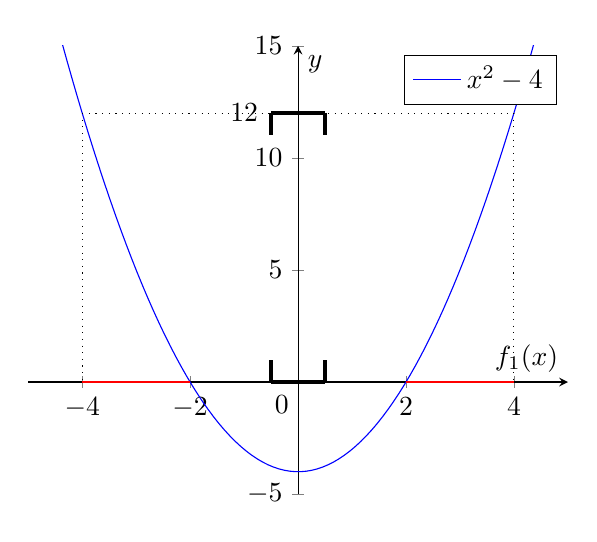
\begin{tikzpicture}
					\begin{axis}[
					    axis lines=middle,
   						xmin=-5,xmax=5,ymin=-5,ymax=15,
						xlabel={$f_1(x)$},
						ylabel={$y$}
]
%Below the positive parabola is defined
					\addplot [
					    samples=100, 
					    color=blue,
]
					{x^2-4)};
					\addplot [
						domain=-4:-2,
					    samples=100, 
					    color=red,
]
					{0};
					\addplot [
					domain=2:4,
					    samples=100, 
					    color=red,
]
					{0};
					\addplot[mark=none, black, dotted] coordinates {(-4,12) (4,12)};
					\addplot[mark=none, black, dotted] coordinates {(-4,12) (-4,0)};
					\addplot[mark=none, black, dotted] coordinates {(4,12) (4,0)};
					\node at (axis cs:-1, 12){12};
					\node at (axis cs:-0.3, -1){0};
					\addplot[mark=none, black, ultra thick] coordinates {(-0.5,12) (0.5,12)};
					\addplot[mark=none, black, ultra thick] coordinates {(-0.5,12) (-0.5,11)};
					\addplot[mark=none, black, ultra thick] coordinates {(0.5,12) (0.5,11)};
					\addplot[mark=none, black, ultra thick] coordinates {(-0.5,0) (0.5,0)};
					\addplot[mark=none, black, ultra thick] coordinates {(-0.5,0) (-0.5,1)};
					\addplot[mark=none, black, ultra thick] coordinates {(0.5,0) (0.5,1)};
					\addlegendentry{$x^2-4$}
				\end{axis}
			\end{tikzpicture}\\
				Für $y=0$:\\
				$$0=x^2-4$$
				$$<=>x^2=4$$
				$$<=>x= \pm 2$$
				Für $y=12$:\\
				$$12=x^2-4$$
				$$<=>x^2=16$$
				$$<=>x= \pm 4$$
				Das heißt, um das Urbild zu bestimmen, wir brauchen alle $x \in [-4,-2]$ und alle $x \in [2,4]$\\
				Also:\\
				$$f_1 \hspace{1pt}^{-1}([0,12])=[-4,-2] \hspace{5pt} \cup \hspace{5pt} [2,4]$$
			\indent d)\\
				\begin{tikzpicture}
					\begin{axis}[
					    axis lines=middle,
   						xmin=-5,xmax=5,ymin=-5,ymax=5,
						xlabel={$x$},
						ylabel={$y$}
]
					\addplot [
					    samples=200, 
					    color=red,
]
					{x^2-4};
					\addlegendentry{$x^2-4$}
				\end{axis}
			\end{tikzpicture}\\
			$f(x)=x^2-4$ ist ein positiver Polynom 2. Grades, also es ist nach unten beschränkt.\\
			\indent e)\\
				$f_1(x)=f_1(-x)$ für alle $x\in\mathbb{R}$, also es ist eine gerage Funktion.\\
				$f_2(x) \neq f_2(-x)$ für alle $x\in\mathbb{R}$, also es ist eine ungerade Fuktion.\\
		\noindent \begin{Large}Aufgabe 4:\end{Large}\\[2pt]
			\indent a)
				$$y=\frac{2x+3}{x+1} => y(x+1)=2x+3=>$$
				$$yx-2x=3-y => x(y-2)=3y=>$$
				$$x=\frac{3y}{y-2}=>$$
				$$f^-1(x)=\frac{3x}{x-2}$$
				$$D_{f^{-1}}=\mathbb{R}\setminus\{2\}$$
			\indent b)
				$$\frac{2\left(\frac{3x}{x-2}\right)+3}{\left(\frac{3x}{x-2}\right)+1}=\frac{\left(\frac{6x}{x-2}\right)+\left(\frac{3(x-2)}{x-2}\right)}{\left(\frac{3x}{x-2}\right)+\left(\frac{x-2}{x-2}\right)}=$$
				$$=\frac{9x-6}{4x-2}=\frac{3(3x-2)}{2(2x-1)}$$
			\indent c)\\
				$f(x)$ ist ein ungerader, negativer Exponent, also es ist immer moton fallend\\
				$$\frac{d}{dx}\left[\frac{2x+3}{x+1}\right]=\frac{(x+1)(2)-(2x+3)(1)}{(x+1)^2}=$$
				$$=-\frac{1}{(x+1)^2}$$
				$$=> f'(x)<0  \mbox{ für alle } \{x \in \mathbb{R} \mid x \neq -1\}$$
				$$=> f_1(x) \mbox{ ist monoton fallend  für }[-1,\infty] $$		
		\noindent \begin{Large}Aufgabe 5:\end{Large}\\[2pt]
			\indent a)
				$$e^{x^2-9}-1=0$$
				$$=> e^{x^2-9}=1$$
				$$=>ln(1)=x^2-9$$
				$$=>x^2-9=0$$
				$$x^2=9$$
				$$x=\{-3,3\}$$
			\indent b)
						$$ln\left(\frac{x^2-4x+3}{x^2-5x+6}\right)$$
						Es müss: $\frac{x^2-4x+3}{x^2-5x+6} >0$\\
						Mit Anwendung der p-q Formel findet man die Nullstellen der beiden Polynome:\\
						$$x_{1,2}=\frac{-p}{2}\pm \sqrt{\left(\frac{p}{2}\right)^2-q}$$
						$$=>x_{1,2}=-\left(\frac{-4}{2}\right)\pm \sqrt{\left(\frac{-4}{2}\right)^2-3}=2 \pm \sqrt{1}$$
						$$=>x_1 = 2+1=3 \hspace{20pt}\mbox{und}\hspace{20pt} x_2 = 2-1=1$$
						$$x_{3,4}=\left(-\frac{-5}{2}\right)\pm \sqrt{\left(\frac{-5}{2}\right)^2-6}= \frac{5}{2} \pm \sqrt{\frac{1}{4}}$$
						$$x_3=\frac{5}{2}+\frac{1}{2}=3 \hspace{20pt}\mbox{und}\hspace{20pt} x_4=\frac{5}{2}-\frac{1}{2}$$
						Wir können zunächst vereinfachen:
						$$\frac{x^2-4x+3}{x^2-5x+6}>0$$
						$$<=>\frac{(x-3)(x-1)}{(x-3)(x-2)}>0$$
						Für $x \neq 3$ darf man beide Terme abkürzen
						$$<=>\frac{x-1}{x-2}>0$$
						Es müss: $x-2\neq 0$, d.h $x \neq 2$\\
						Die Ungleichung gilt nur dann, wenn beide Terme entweder positiv oder negativ sind\\
						1.Fall $x>1$ und $x>2$ d.h $x>2$:
							$$L_1=]2,\infty[$$
						2.Fall $x<1$ und $x<2$, d.h $x<1$:
							$$L_2=]-\infty,1[$$
						Daraus folgt:\\
						$$L=L_1\cup L_2 = ]-\infty,1[ \hspace{5pt} \cup \hspace{5pt} ]2,\infty[$$
						Somit $D_{f_2}=\mathbb{R}\setminus\{[1,2]\}$						
\end{document}